\section{Introduction to electrochemistry}

In this part of the course we want to put into practice the concepts obtained during the theoretical study of the kinetic inside a material and understand how to use it in practice. Our main focus will be the creation and conservation of energy inside batteries or, as chemists call them, \textbf{electrochemical cells}. Therefore, we will start with a simple introduction to the main concepts needed in this study.

The concept behind a battery is trivial in some sense, basically only three things needs to be present to have a working device: two or more electrodes, an electrolyte, and an external circuit. The idea is the one of using redox reactions between the electrodes, usually composed by metals or semiconductors, to make electron travel inside the circuit. In practice, let's imagine using two bars of \ce{Zn} and \ce{Cu} as electrodes putted inside a liquid, the two of them can give rise to a total cell reaction where electrons travel from Zinc to Copper as follows
\begin{equation}
    \ce{Zn_s + Cu_l^{2+} -> Zn_l^{2+} + Cu_s},
\end{equation}
where the subscripts tell the phase in which the atom is present. Basically, what is happening is that two different reactions are performed inside the system: one where the Zinc looses two electrons giving rise to the positive ion, and one where ionic Copper takes those two electrons. Therefore, the former is an \textbf{oxidation} reaction, while the latter is a \textbf{reduction} one, generating a distinction to keep in mind.
\dfn{Oxidation-Reduction}
{
    Inside an electrochemical cell the element is reducing if is gaining electrons in the process, while is oxidizing if is loosing electrons.
}
\noindent
Also, during the course we will call the element that undergo oxidation as \textbf{anode}, while the one reducing will be the \textbf{cathode}. Still, the aim of our device is creating this reaction and using the electrons that are generated in the process. So that the point is, we connect the anode and cathode with a circuit, so that electrons will start to spontaneously flow from one to the other generating the following semi-reactions
\begin{align}
    &\ce{Cu_l^{2+} + 2e^- -> Cu_s}, &\ce{Zn_s -> Zn_l^{2+} + 2e^-}.
\end{align}
This process will so generate a current in the circuit, meaning that a voltage, called \textbf{cell potential}, is present between the two electrodes giving us energy that we can use. That is all great but as the reaction goes on the density of \ce{Zn^{2+}} around the anode will reach saturation slowing down the reaction, a problem that can be easily eliminated by using the electrolyte. 
\begin{figure}
    \centering
    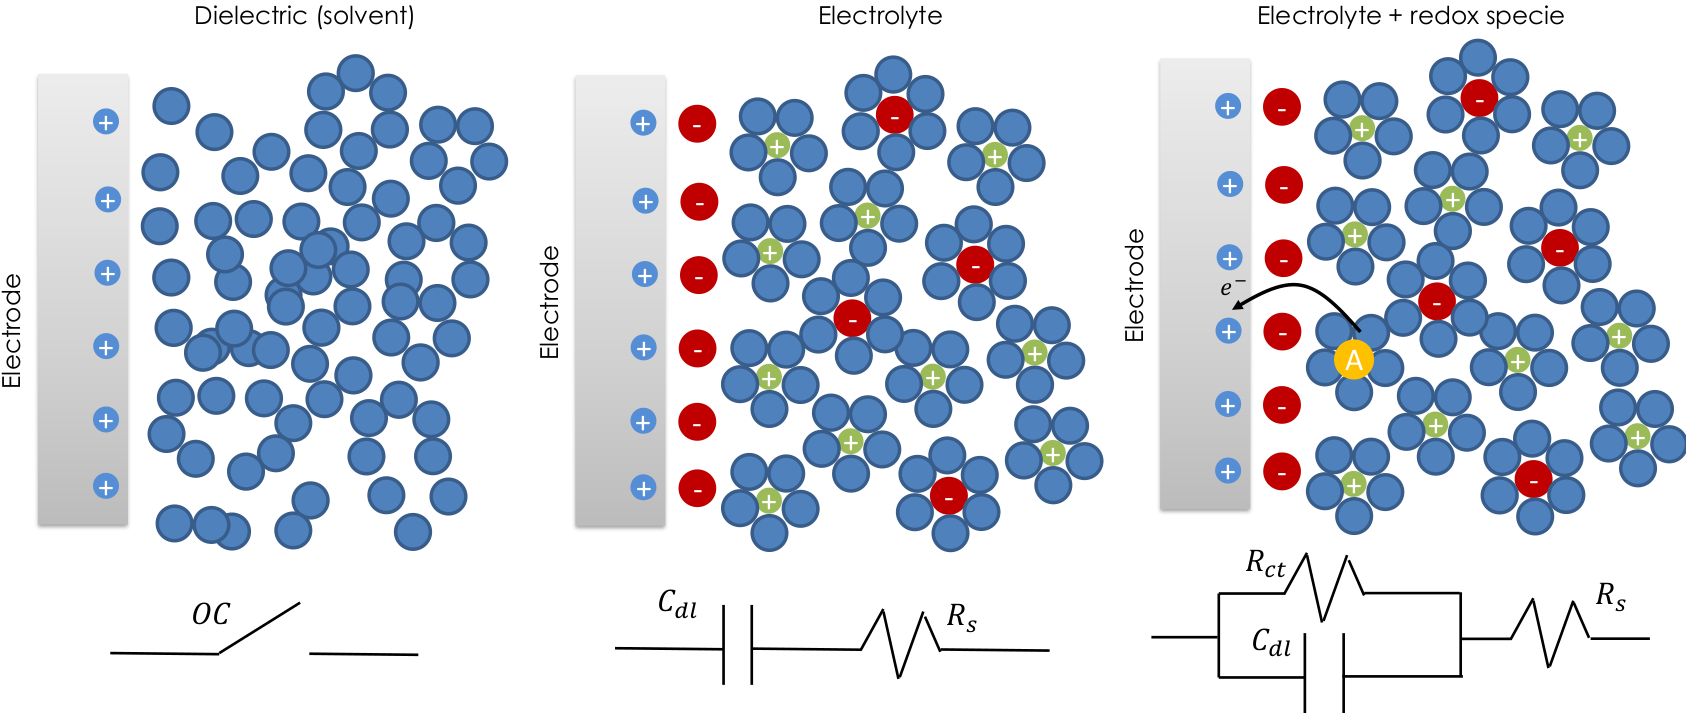
\includegraphics[width=0.9\textwidth]{Immagini/ElettrolitaEs.png}
    \caption{
        Graphical explanation of how an electrolyte works in practice, showing how the presence of ions inside it allows for the charge to move in the solution making species travel from anion to cathode making the reaction continue. Also, every step can be represented as a different circuit.
    }
    \label{fig:ElettrolitaEs}
\end{figure}
In fact, as we can see in \figref{fig:ElettrolitaEs}, the electrolyte has the task of letting the ions generated move inside the system. For example, if a salt is present in the solution, the latter will split generating positive and negative ions which will travel to the cathode and anode respectively. That will give rise to a system that looks like a capacity, where the ions move as long as the charge around the electrodes is not compensated, but if inside the electrolyte we place also the redox species, \ce{Cu^{2+}}, they will not only move to the electrodes but will react with those keeping the reaction going. For this reason the choice of the electrolyte is really important, since the diffusion properties of ions inside it will be key to the output power that we can have.

The final result that we obtain by this construction is a device that is able to generate a voltage and a current density inside the circuit attached to it. Still, the voltage and the current generated are not really as we might expect them to be. Usually, current and potential are linearly related via Hom's law, but here the relation between current density and cell potential is not, showing also the equilibrium point with no current $\vb{J} = 0$ at $\Delta V \neq 0$, as we can see in \figref{fig:CellCaracteristic}. Such a peculiar behavior can be described by the fact that simply the potential generated by the cell is not simply given by electrostatic interactions but a complex series of interfaces and chemical phenomena enters to play arising two questions: how to define the potential in electrochemistry, and what properties are affecting the current-potential characteristic?
\begin{figure}[t]
    \centering
    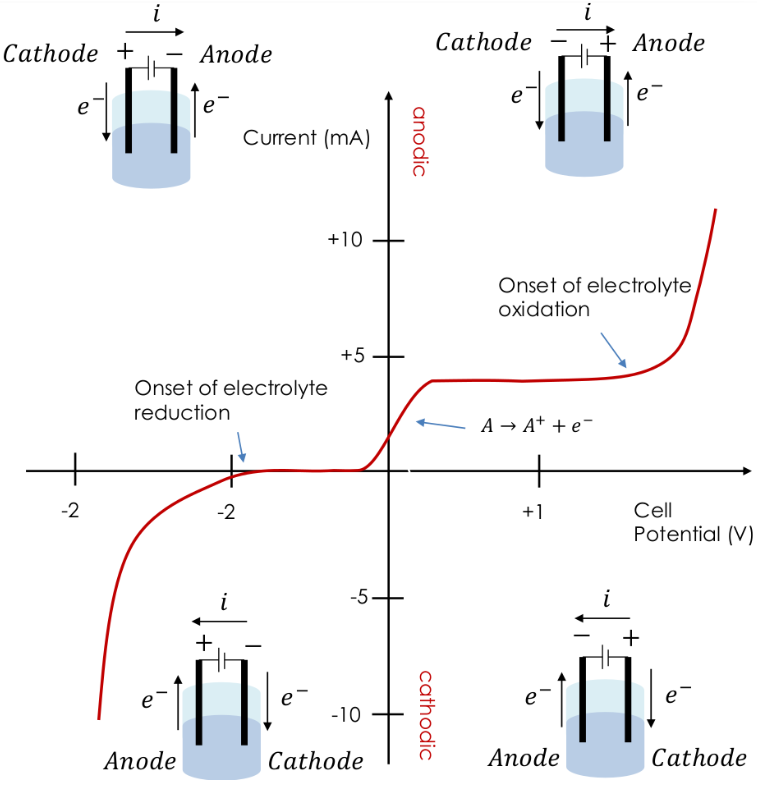
\includegraphics[width=0.4\textwidth]{Immagini/VvsI.png}
    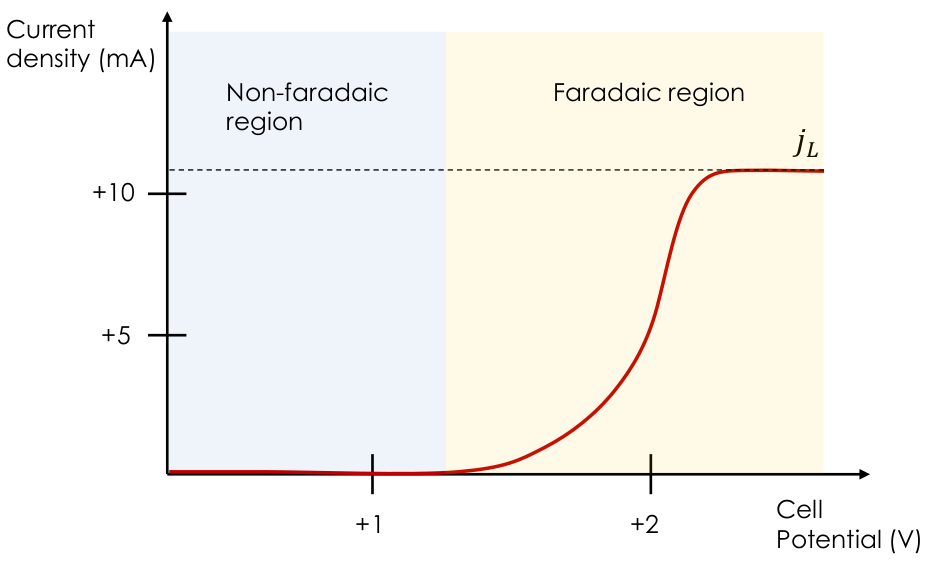
\includegraphics[width=0.58\textwidth]{Immagini/CarRegions.png}
    \caption{
        Graphics of the characteristic of a general electrochemical cell, with a close up on the first, and most important, quadrant. In the first quadrant we can see how the current will reach a plateau in the last part, that is due to the presence of diffusion inside the system that limits the speed at which the electrons can be emitted.
    }
    \label{fig:CellCaracteristic}
\end{figure}
Both of the questions will be answered during this last part of the course, but we will try to give a simple explanation for the second one right now.

First, we should consider how inside the I-V characteristic showed in \figref{fig:CellCaracteristic} the current density increase suddenly to then reach a plateau. That is our range to work with it, basically having a constant supply of current is exactly what we want from a battery, also if we would to go further the current will start to grow exponentially. That is due to reaching a value of the potential in the cell that is able to generate redox also inside the electrolyte oxidizing it, and is something that we want to avoid. Therefore, we will focus on the first part of the curve in the first quadrant, as showed in the figure on the right of \figref{fig:CellCaracteristic}. Inside that window we can identify two main regions to work with:
\begin{itemize}[align=left, leftmargin=*]
    \item[\textbf{Non-Faradic.}] The first part where no current is present since the charge is accumulating near the electrodes as a capacitor charging. Possible presence of small capacitive current;
    \item[\textbf{Faradic.}] The current becomes proportional to the reaction rate and starts to grow rapidly. 
\end{itemize}
The latter region is the interesting one, and we can see how the first part, called \textbf{activation control}, shows an exponential growth of the current since the reaction starts and the electrons are generated with speeds proportional to the potential. Meaning that in this reagion a lot of factors, like: catalytic properties of the surface, area, adsorption, and concentration of species, are all important to the determination of the power supplied. Then, a rapid growth happens, and the constant current is reached in a situation called \textbf{mass-transport control}. The latter is a region of the graph where $J$ is dictated by the velocity of diffusion inside the electrolyte, since the electrons goes much faster than the ionic species needed to make the reactions the numbers of electrons per unit time that pass through the circuit is limited by the flux of ions. Therefore, the current in the two regions can be described by
\begin{align}
    &J_{ac} = nFk_{ct}c_x, &J_{mt} = nFDc_b,
\end{align}
where $F$ is the charge inside one mole of electrons, and $n$ the moles generated. Then, also the region in between, called \textbf{Mixed control} can be easily described using these two results since it's a mixture of the two often approximated with
\begin{equation}
    \frac{1}{J} = \frac{1}{J_{ac}} + \frac{1}{J_{mt}}.
\end{equation}
In this way we can understand how the choice of the electrolyte is really important, since it's diffusion properties will determine the current density generated in the electrochemical window of the device.

\ex{Lead-Acid Battery}
{
    A good example of battery that we can look at just a moment is the \ce{Pb} one, where the anode and cathode are created by bars of pure \ce{Pb} and \ce{PbO_2} with an acid electrolyte. The reaction that happens inside the system are
    \begin{align*}
        &\ce{Pb + SO_4^{2-} -> PbSO_4 + 2e^{-}},\\ 
        &\ce{PbO_2 + SO_4^{2-} + 4H^+ + 2e^{-} -> PbSO_4 + 2H_2O},
    \end{align*}
    Then, imagine that we use the battery for an hour at a constant current of \SI{20}{A}, we can compute the amount of lead needed to sustain such power supply. The charge that is transported is $Q = It$, where we know both of them having that \SI{72000}{C} is effectively transported from anode to cathode, meaning $n_e = Q/F = \SI{0.746}{mol}$. Therefore, we can compute the moles of lead needed to generate such amount of electrons by using the first semi-reaction and see how
    \begin{displaymath}
        n_{Pb} = n_e/2 = \SI{0.373}{mol} = \SI{154.5}{g},
    \end{displaymath} 
    not a small amount due to the high weight of lead. For that reason the Lithium batteries seems better, \ce{Li} is lighter needing less weight for the same amount of power.
}
\nt
{
    The most used types of electrolytes are liquid where salt is inserted in order to generate ions that can freely move inside. In this way a high mobility is achieved, but a large research is present in this field, especially to create efficient solid state electrolytes with high enough diffusivity to work nicely and also reduce the problematics related to using liquids, such as safety due to flammability. By now some solid state devices are used but since $D$ increase with temperature are mainly used for particular application where we need to work in hot systems.
}

\subsection{Thermodynamics of an electrochemical cell}

After this long introduction we can try to dig in the thermodynamics of the system and try to set up the basis for the discussion of specific devices. The first thing that we need to define is the concept of reversibility, which in electrochemistry is slightly different from the one we expect. The idea is that when performing an electrochemical reaction we can evaluate the value of the voltage between electrodes in the equilibrium state $V_0$ and then, if the reaction is \textbf{reversible}, we are able to promote either the forward and reverse reaction by applying a positive or negative bias to the system. In this sense we can give a really simple and general definition for the reversibility of a reaction as follows.
\dfn{Microscopic reversibility}
{
    Infinitesimal change in a driving force causes the reaction to reverse direction.
}
\noindent
This definition is intrinsically different from the real thermodynamic definition of reversible, but we can see how they are related somehow. In particular, a chemical reaction that is irreversible in this sense is also thermodynamically irreversible, but if is reversible is not sad to be reversible in the real sense. Still, in general all of this is thought in terms of reaction rates for reversible reactions, having that if the rate of advancing $K_a$ and going back $k_b$ are nearly equal is reversible, if instead $k_a \gg k_b$ than is irreversible. Basically, you only need to thing in terms of $k$ in a reaction to say if it is reversible or not.

Knowing that we can start by thinking about the main quantities that will play a role inside the thermodynamic of the system, and since I would not like to stay here and describe one by one a series of tedious definition I will report the table given in the slides in \tabref{tab:Def}.
\begin{table}[t]
    \caption{
        Table with definition of all the types of variables we are going to use in this study and so on.
    }
    \label{tab:Def}
    \centering
    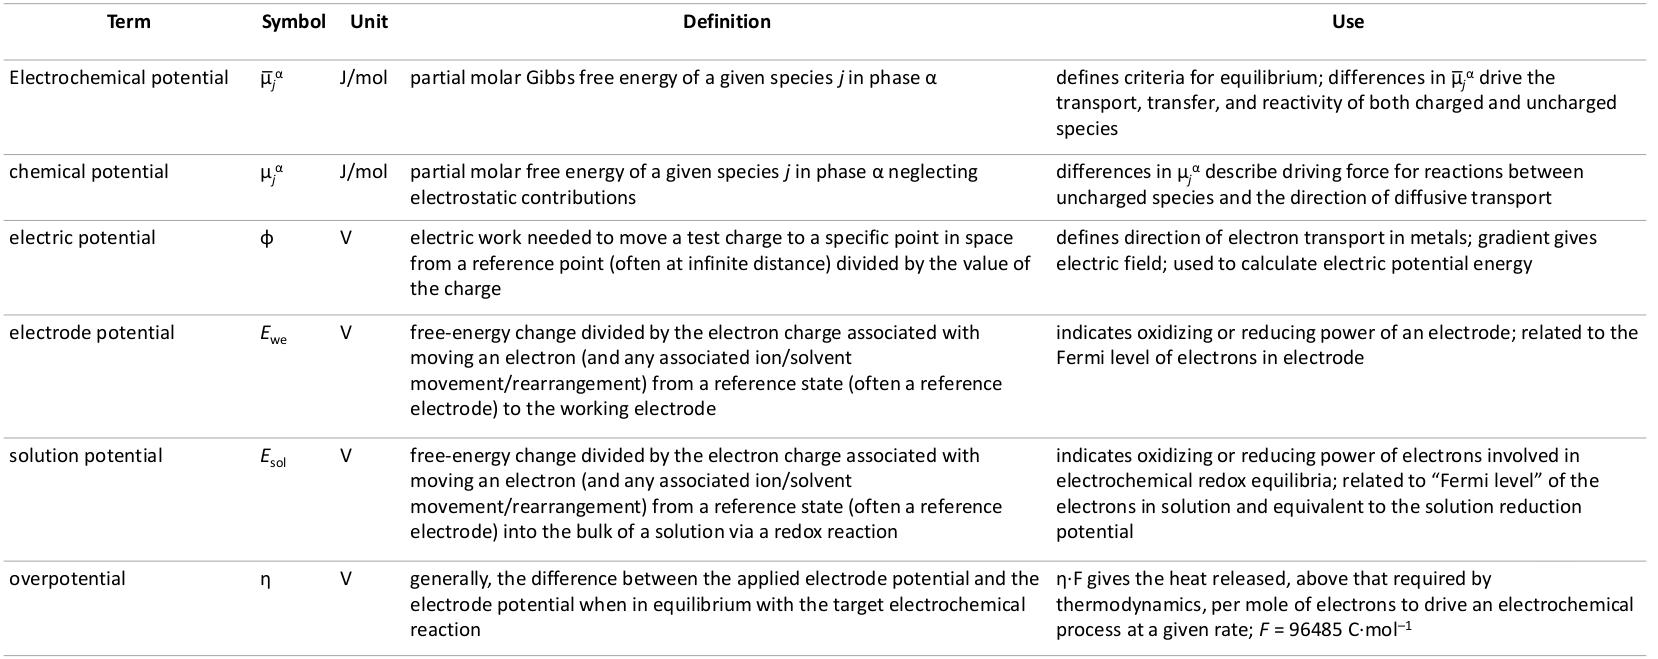
\includegraphics[width=0.9\textwidth]{Immagini/TabDef.png}
\end{table}
With the latter we can a more into the thermodynamic of the system and see how the flux that defines the direction of the reaction looks like in this context. Let's take the chemical potential of component $i$ to write down the following relation as the flux of that component
\begin{equation}
    \vb{J}_i = -\left( \frac{c_iD_i}{RT} \right)\grad \mu_i,
\end{equation}
where the chemical potential of a specie in solution will be defined as
\begin{align}
    &\mu_i = \pdv{G}{n_i} = \mu^0_i + RT\ln(a_i), &a_i = \gamma_i(c) c_i.
\end{align}
Basically, the potential the same as we have already seen, with the activity coefficient present. Still, this definition does not take into account the electrostatic effect presents, that we can insert by using the potential per mole in phase $\alpha$ called $\phi^\alpha$. 
\dfn{Electrochemical potential}
{
    The chemical potential of the $i$-th component of an electrochemical system needs to take into account also the electric potential per mole in the phase $\alpha$ in which is present, $\phi^\alpha$, giving
    \begin{equation}
        \label{eq:ElecPotDef}
        \overline{\mu} = \mu_i + z_i F \phi^\alpha,
    \end{equation}
    where $z_i$ is the charge number on the specie we are looking at.
}
\noindent
That is the real potential we are going to use, so that the condition on the equilibrium of the system is given in terms of $\overline{\mu}$ and not simple $\mu$. For this reason even if all the electrochemical potential of the species are equal still we can have differences in electrical potential, generating potential differences even at equilibrium called cell potential. Also, it's interesting to see how inside the definition of \eqref{eq:ElecPotDef} we have how the chemical potential describe the short-range interactions while the electrical part counts for the long range since
\begin{align}
    &\mu_i \propto r^{-6}, &z_iF\phi^\alpha \propto r^{-1}.
\end{align}
Therefore, we can have one component that wins on the other in specific situations, but still the two are strictly related. In particular, the real measurable quantity is $\overline{\mu}$ it's not possible to evaluate $\mu$ or $\phi$ separately since the measure of a potential always imply the creation of an interface during the measurement having both in the final result.

The new definition of $\overline{\mu}$ can be put at use in a really simple way. For example, we can imagine taking a metal and apply a potential on it so that the electrochemical potential difference of the electron in two different positions of the material becomes
\begin{equation}
    \Delta \overline{\mu}_e = \overline{\mu}_e^\alpha - \overline{\mu}_e^\beta = \mu_e^\alpha - zF\phi^\alpha - \mu_e^\beta + zF\phi^\beta = -zF\Delta\phi.
\end{equation}
Where we assumed that the chemical potential of the single electron remained equal inside the metal. Using this result we can see how the flux of electron can be written as
\begin{equation}
    \vb{J}_e = - \left( \frac{c_eD_e}{RT} \right)\grad \overline{\mu}_e = zF\left( \frac{c_eD_e}{RT} \right)\grad \phi = R\grad \phi,
\end{equation}
the Hom's law was simply found. Still, this is only a trivial application what we want to do is studying what happens when two metals touching each others in equilibrium. Where we can easily see how the following becomes true.
\thm{Interface potential}
{
    When two metals $M_1$ and $M_2$ are in contact with each others a potential difference appear at equilibrium in the interface of the two solid phases given by
    \begin{equation}
        \Delta \phi^{M_1-M_2} = \frac{\Delta \mu^{M_1 - M_2}_e}{zF}.
    \end{equation}
}
\pf{Proof}
{
    That is incredibly easy, you only need to recall how the equilibrium condition in this case become $\overline{\mu}_e^{M_1} = \overline{\mu}_e^{M_2}$ so that you place them equal and obtain the result.
}
\noindent
Therefore, using the electrochemical potential is really helpful in the study of how the chemistry of the system mix with its electrical properties. For this reason it's the main quantity that we are going to study inside batteries, and we can predict cells behaviors with that.

\subsection{Interface at equilibrium}

To understand how the electrochemical cell works properly we need first to develop a way to study how solid liquid interface works in general, since the cell is composed by two metal electrodes inside a liquid electrolyte in general. We have already seen what happens with solid-solid interface, but now we aim to look more into the equilibrium of a reduction reaction like
\begin{equation}
    \ce{O + ne^-(M)} \rightleftharpoons  \ce{R}.
\end{equation}
In such an equation we can easily find out the potential difference generated by the transport of electrons at equilibrium by the following important result.
\thm{Nernst equation}
{
    The electrode potential generated by a redox reaction at equilibrium $E$, depend both on ambient condition and chemical properties of the system through the relation
    \begin{equation}
        E = E^0_{O/R} + \frac{RT}{nF}\ln(a_O/a_R),
    \end{equation}
    where $E^0_{O/R}$ is also called standard electrochemical potential.
}
\pf{Proof}
{
    we can start by setting the equilibrium by doing the following operation
    \begin{equation}
        \Delta \overline{\mu}_e = \overline{\mu}_R^s - (n\mu_e^M + \mu_O^s) = 0,
    \end{equation}
    where the up scripts $s$ and $M$ tells us if the element is in the electrolyte solution or in the solid component. Then, by using the definition of electrochemical potential and the fact that $z_R = z_O - n$ with $z_e = -1$ we can obtain
    \begin{equation}
        \label{eq:potentialAtSolidLiquidInterface}
        z_OF(\phi^s - \phi^M) = (\mu_R^s - \mu_O^s) - n\mu_e^M,
    \end{equation}
    where the contributions from electrostatics, chemistry of the solution and the one of the solid were divided. We can now use the fact that $\mu_i = \mu_i^0 + RT\ln a_i$ to retain the following form
    \begin{equation}
        -\frac{z_O}{n}(\phi^s - \phi^M) = -\frac{\mu_R^{0,s} - \mu_O^{0,s}}{nF} + \frac{\mu_e^M}{F} + \frac{RT}{nF}\ln(a_O/a_R).
    \end{equation}
    Here we can finish the job by defining the two main variables in the Nernst equation as follows
    \begin{align}
        &E = -\frac{z_O}{n}(\phi^s - \phi^M), &E^0_{O/R} = -\frac{\mu_R^{0,s} - \mu_O^{0,s}}{nF} + \frac{\mu_e^M}{F} = -\frac{\Delta G^0}{nF}.
    \end{align}
    This also shows how the standard potential is also related to the form of the free energy difference.
}
\noindent
That is a powerful result, but still works only at equilibrium and understand when interfaces are at equilibrium may not be so easy. We can generally say that if the charge transfer kinetics is very fast we can be in Nernstian conditions since the superficial activity rapidly equilibrates before mass.

Now, we can imagine to level up and take into account a full cell composed by two electrodes in an electrolyte solution, so that two redox happens one for $M_1$ and one for $M_2$. Now, in order to work better with our system we are going to assume that the electrolytes solutions are separated by a porous material that allows still for charge equilibrating still avoiding the contamination of reactants.  In this way the electric potential in the solution $\phi^s$ is constant so that by writing the $\Delta \overline{\mu}$ for both reaction and sett equilibrium we obtain \eqref{eq:potentialAtSolidLiquidInterface} for both metals which can be summed up in order to obtain
\begin{equation}
    \label{eq:potentialInACell}
    -z_{O2}F(\phi^M - \phi^{M2}) = \frac{z_{O2}}{z_O}(\mu_R^s - \mu_O^s) - z_{O2}\mu_e^M - (\mu_{R2}^s - \mu_{O2}^s) + z_{O2}\mu_e^{M2}.
\end{equation}
By assuming that $\mu_e^M = \mu_e^{M2}$ we can obtain a form of the potential between the electrodes, that is generated by the cell, depending on the chemical properties of the two semi-reactions present inside the cell. In particular, if we define the cell potential $E_{cell}$ to be that potential energy difference we can transform \eqref{eq:potentialInACell} into
\begin{equation}
    E_{cell} = E_{right} - E_{left}.
\end{equation}
Meaning that if we know the variation of the potential at the interface for the single reactions we can compute the total one. In particular, we can also have a look at how this knowledge can be used inside in order to evaluate the free energy difference of the reaction as follows.
\thm{Gibbs and electrode potential}
{
    inside an electrochemical cell the variation of free energy of the system is proportional to the electrode potential following the relation
    \begin{equation}
        \Delta G = -nF E_{cell}.
    \end{equation}
}
\pf{Proof}
{
    For a generic reversible reaction in a closed system the maximum amount of work that can be extracted from the cell is $\Gamma = -W_{chem}$. If that work is extracted through heat dissipation we can say that the chemical work is equal to the electrical one, which is given by the simple relation
    \begin{equation}
        W_{el} = nFE_{cell}.
    \end{equation}
    Which is the work done on every moving charge present, completing the result.
}
\noindent
That is great, since that tells us that if $E_{cell}>0$ than the reaction is spontaneous. Meaning that only by looking at the components used in the cell and their reduction potentials, since the energies $E$ are referred to the reduction reaction $\mu_R - \mu_O$, we can tell not only what $E$ will be, but also in which direction it will point.

The fact that the potential is strictly related to the free energy allows us also to write down another important relation that generalize Nernst equation and probably is the real version for physicist.
\thm{Generalized Nernst equation}
{
    Consider a generic reaction at equilibrium $\ce{n_{R_1}R_1} + \dots \ce{->} \ce{n_{P_1}P_1} + \dots$ we can write down the electrode potential of the cell using
    \begin{equation}
        E_{cell} = E^0_{cell} + \frac{RT}{nF}\ln\left( \frac{\prod_i a_{R_i}}{\prod_i a_{P_i}} \right).
    \end{equation}
}
\pf{Proof}
{
    Basically we know how the change in free energy can be written up using the chemical potentials as
    \begin{equation}
        \Delta G = \sum_i n_{P_i}\mu_{P_i} - \sum_i n_{R_i}\mu_{R_i}.
    \end{equation}
    Then we can recall the form of the chemical potential $\mu = \mu^0 + RT\ln a$ to obtain directly the final form by dividing by $-nF$.
}
\noindent
That will allow to compute the cell potential also in the case of more complex reactions, which is really important for applications. Still this formula imply that we know the values of the reduction potential of all the elements in the reaction, meaning that we need to understand how to evaluate them. The latter is not a trivial task, since if we want to evaluate the potential at an interface directly I need to insert in the system a third element, a voltmeter, which creates a new interface modifying the properties. The idea is, therefore, to place the electrode of which we want to evaluate the potential, called \textbf{working electrode} (WE),  inside a cell where the other electrode is a standard reference, \textbf{reference electrode} (RE). So that, we can evaluate $E_{cell}$ by simply measuring the one between electrodes and then obtain the final result
\begin{equation}
    E_{WE} = E_{cell} + E_{RE}.
\end{equation}
In order for such measurement to be precise we will need for the RE to possess the properties of an \textbf{ideal non-polarizable electrode}, meaning that the value of $E_{RE}$ does not depend on the bias applied to the system. The latter usually comes from a third electrode called \textbf{counter electrode} (CE), from which a current is inserted in the circuit in order to flow from CE to WE, RE is only used for potential measurement. Therefore, to construct a good RE, that has a constant potential not varying with change in the applied current, is often composed by a metal wire in a solution containing a redox couple providing:
\begin{enumerate}[label*=\protect\fbox{\arabic{enumi}}]
    \item Reversible reaction with fast kinetics, allowing the use of Nernst equation;
    \item Essentially constant composition;
    \item Ionic conduction to close the electrochemical circuit.
\end{enumerate}
A good example of such reference electrodes is the hydrogen one, which is generally used as standard having a potential sett to $E^0 = \SI{0}{V}$.

\nt
{
    He also showed a particular type of diagram that can be used in order to study redox reaction called Pourbaix diagram, which simply is a phase diagram for the reduction of one electrode in the cell as a function of pH of the solution and equilibrium potential, $E_{cell}$.
}

\ex{Cu/Fe-H cell}
{
    We have made a simple example taking looking at the values of the potential generated by a Cu-H cell and a Fe-H cell. To do that you need to look at an online table and search for the semi-reaction to find out how
    \begin{align*}
        &\ce{Cu^{2+}(aq) + 2e^-_M -> Cu(s)}, &E^0 = \SI{+0.340}{V},\\
        &\ce{Fe^{2+}(aq) + 2e^-_M -> Fe(s)}, &E^0 = \SI{-0.440}{V},\\
        &\ce{H_2^{2+}(aq) -> 2H^+ + 2e^-}, &E^0 = \SI{+0.000}{V}.\\
    \end{align*}
    Combining them we can find out the cell potentials for the two complete electrochemical reactions as
    \begin{align*}
        &\ce{Cu^{2+} + H_2 -> Cu + 2H^+}, &E^0 = \SI{+0.340}{V},\\
        &\ce{Fe^{2+} + H_2 -> Fe + 2H^+}, &E^0 = \SI{-0.440}{V}.\\
    \end{align*}
    Meaning that the reduction of Copper is spontaneous, while the one of Iron requires energy since naturally it will oxidase.
}